\section{Imports \& Exports}


%%%%%%%%%%%%%%%%%%%%%%%%%%%%%%
\subsection*{Cell Imports}
\textit{Successively: static import; multiple cells; with dependency injection; aliasing; non-public.}\\
\cde{import \{chart\} from '@mbostock/phases-moon'}\\
\cde{import \{chart, viewof year\} from \dots}
\cde{import \{chart\} with \{mydata as data\} from \dots}\\
\cde{import \{chart as barchar\} \dots}\\


\textit{Note: Imported cells evaluate dependencies without binding them to the local notebook. Bindings are live ($\Delta$ with underlying dependencies), but lazily evaluated.}
%\begin{comment}\begin{wrapfigure}[2]{r}{10mm}
%\vspace{-4mm}
%\resizebox{10mm}{!}{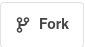
\includegraphics[]{img/fork.jpg}}
%\end{wrapfigure}\end{comment}
\textit{Since you can only import \textbf{named} cells, consider ``forking'' a notebook instead.}\\


%%%%%%%%%%%%%%%%%%%%%%%%%%%%%%
\subsection*{\href{https://observablehq.com/@observablehq/introduction-to-require}{Require}}
\textit{Used for plain JavaScript library imports.}\\
\entry{43mm}{mmnt = require("moment")}{\href{https://momentjs.com/}{moment} lib}\\
\entry{43mm}{mmnt = require("moment@2")}{vers. 2}\\
\entry{43mm}{ab = require("a", "b")}{multiple $\to$ 1}\\

\textit{Libs fetch from \href{https://www.npmjs.com/}{npm} by default. Override like:}\\
\entry{49mm}{d3 = require("my.server/d3.js")}{www loc}\\
\entry{49mm}{d3 = require("localhost/d3.js")}{local}\\

\textit{As an alternative, consider \href{https://exploringjs.com/es6/ch\_modules.html}{ES6-native imports}:}\\
\cde{d3\_esm = import(\textquotedbl https://some.cdn/d3@6\textquotedbl)}\\


%%%%%%%%%%%%%%%%%%%%%%%%%%%%%%
\subsection*{Sharing}
\textit{Notebooks default to ``private'' access but can also be ``shared'' (exposing an obfuscated url) or ``published,'' all as available in the UI. Alternatively, click to left of a cell to download its contents to png or json, etc.}


%%%%%%%%%%%%%%%%%%%%%%%%%%%%%%
\subsection*{\href{https://observablehq.com/@observablehq/introduction-to-embedding?collection=@observablehq/embedding-notebooks}{Embedding}}
\textit{To the left of a cell, select ``embed'' to generate copy-pasteable html }\texttt{IFrame}\textit{ code (which will, in turn, include the observable runtime). \href{https://observablehq.com/@jashkenas/handy-embed-code-generator}{Here} is a tool that generates an IFrame for multiple cells. Alternatively, download a zip archive of project contents by clicking ``download code.'' The generated archive is described \href{https://www.tophtucker.com/observable-docco/index.js.html}{here}. Even better, just install it via npm using the url in the download code menu option:}\\
\cde{unix-shell\$ @observablehq/runtime}\\
\cde{unix-shell\$ npm install \textquotedbl <url>\textquotedbl}


%%%%%%%%%%%%%%%%%%%%%%%%%%%%%%
\subsection*{\href{https://observablehq.com/@observablehq/downloading-and-embedding-notebooks}{Observable Runtime}}
{\it A {\rm \href{https://github.com/observablehq/runtime}{\cde{Runtime}}} instance can spawn a {\rm\tt \cde{module}}, which, when passed an {\rm \href{https://github.com/observablehq/runtime#modules}{\cde{observer}}}, spawns a {\rm \href{https://github.com/observablehq/runtime#variables}{\cde{variable}}}, which is a piece of state in a reactive program. The standard observer is {\rm\tt \href{https://github.com/observablehq/inspector}{\cde{Inspector}}}, which renders the current value of the given variable to its associated DOM element.}

\cde{<html><body><script type=\textquotedbl module\textquotedbl>}\\
\cde{import \{Runtime, Inspector\} from \dots}\\
\cde{import define from \textquotedbl https://\dots\textquotedbl;}\\
\cde{const runtime = new Runtime();}\\
\cde{const main = runtime.module(define, }\\
\cde{ \phantom{xxx} name => \{ if (name === \textquotedbl hello\textquotedbl) \{ }\\
\cde{ \phantom{xxxxxx} return new Inspector(document.body);}\\
\cde{ \phantom{xxx}  \} }\\
\cde{\});}\\
\cde{</script>}\\